\documentclass[conference]{IEEEtran}
\usepackage{url}
\usepackage{graphicx}
\usepackage{subfigure}

\begin{document}

\title{The GHTorrent dataset and tool suite}

\author{\IEEEauthorblockN{Georgios Gousios} 
\IEEEauthorblockA{
Software Engineering Research Group\\
Delft University of Technology\\
Delft, The Netherlands\\
Email: g.gousios@tudelft.nl}
}

\maketitle

\begin{abstract}
Foo
\end{abstract}

\begin{IEEEkeywords}
Git, pull request, collaborative development
\end{IEEEkeywords}

\section{Introduction}
During the recent years, Github has been taking 

\begin{figure}
  \begin{center}
    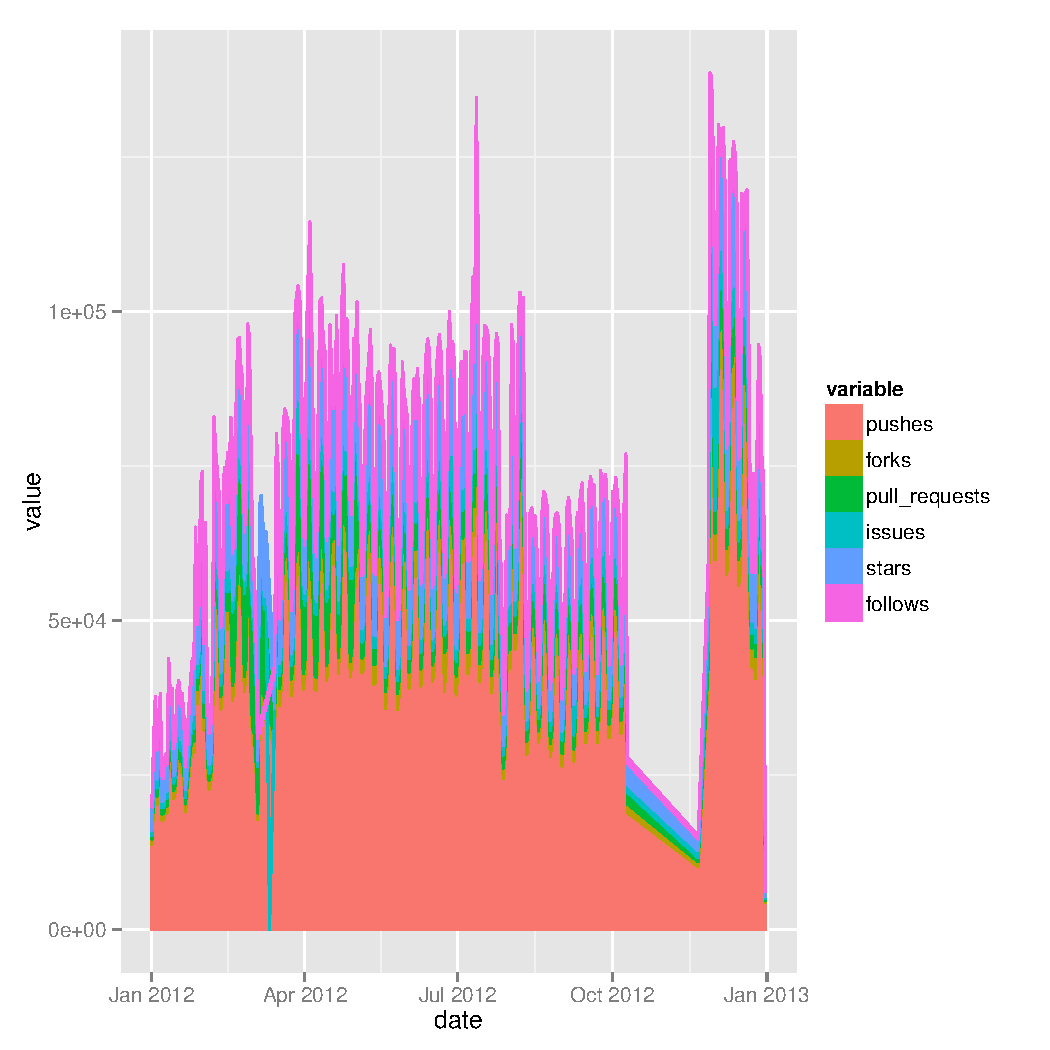
\includegraphics[scale=0.3]{github-growth}
  \end{center}
  \caption{Github's growth in terms of emitted events}
  \label{fig:growth}
\end{figure}

The proposed data collection scheme was first presented in~\cite{GS12}.
Since this work, the data collection process has been fully
implemented, the data schema has been stabilized and a new service
to collaboratively collect and query the data has been implemented.
In this paper, we focus on the newest developments and present
characteristics of the dataset to 

\section{Data schema}

\begin{table*}
  
  \begin{center}
    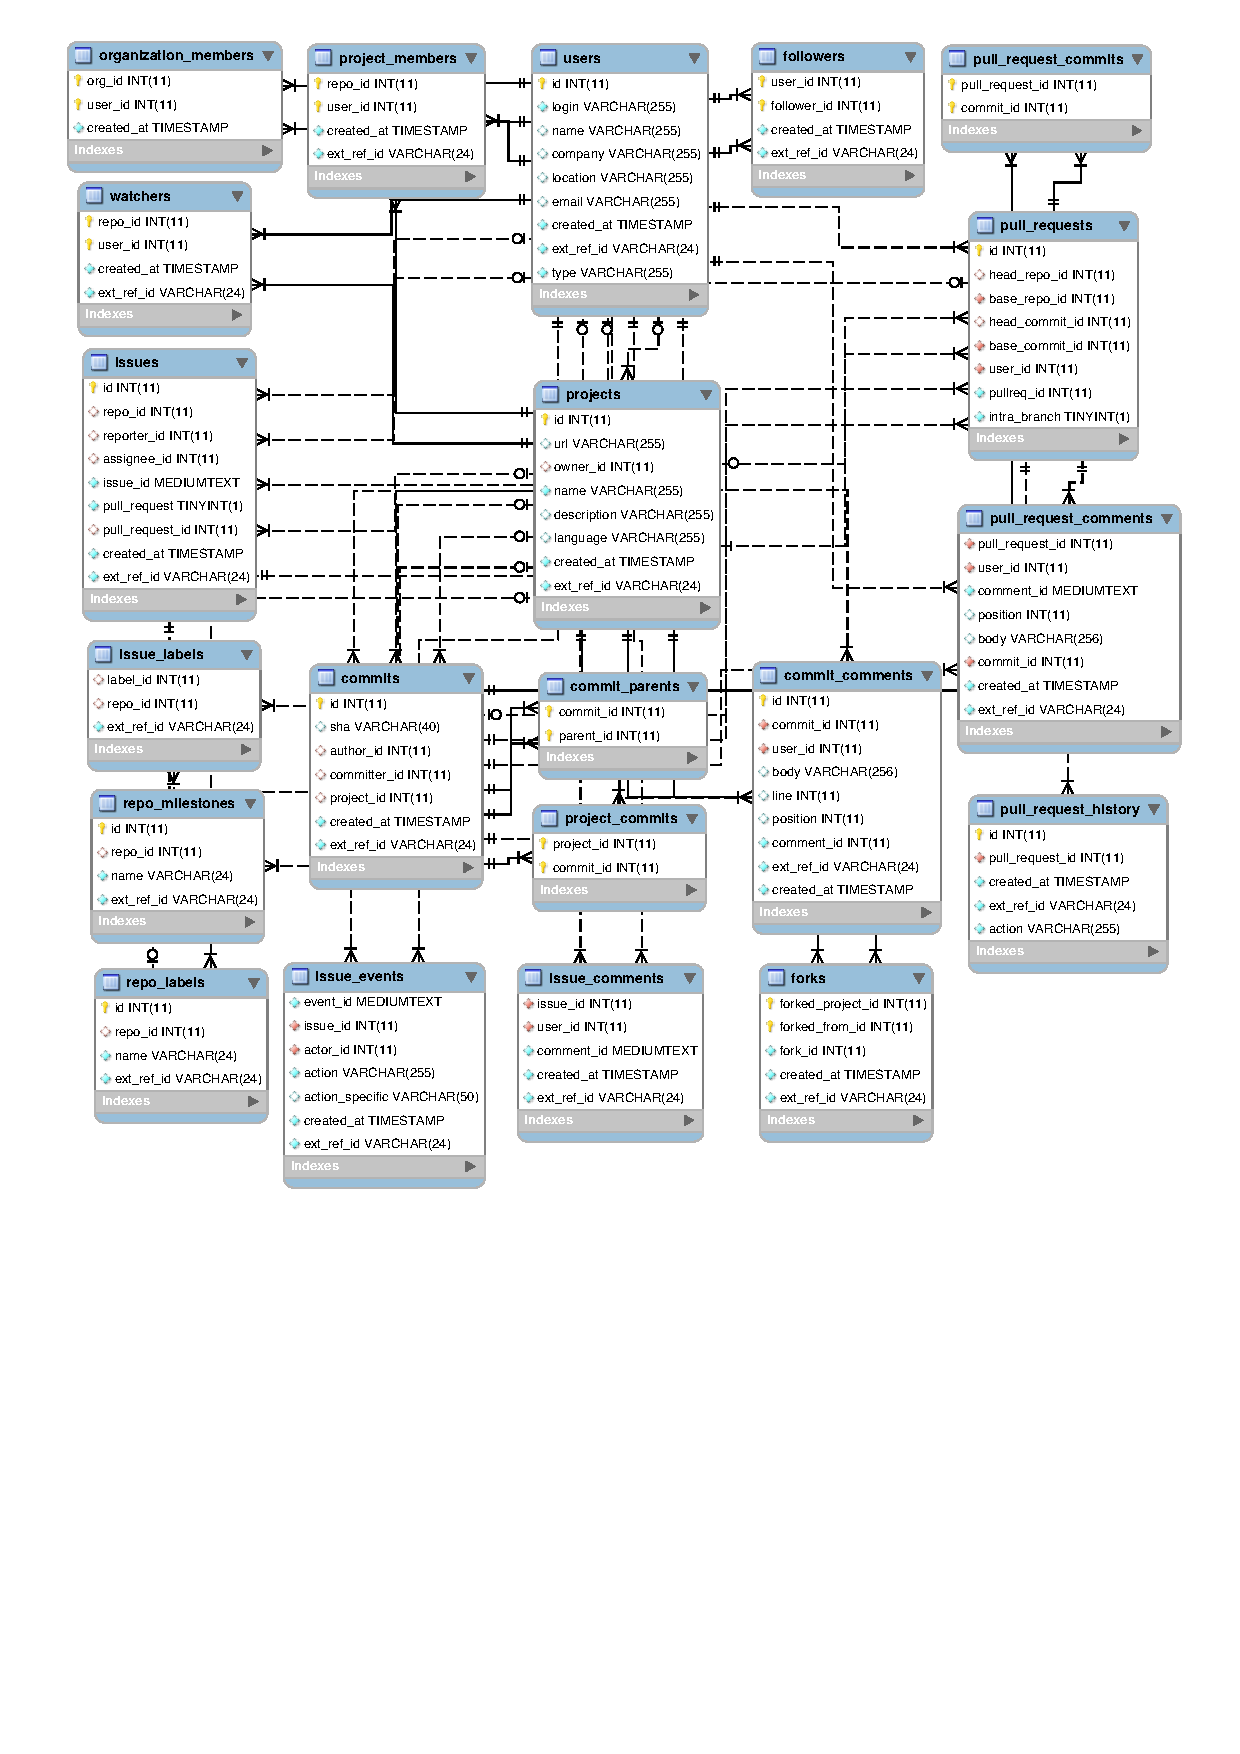
\includegraphics[scale=0.6]{ghtorrent-schema.pdf}
  \end{center}
  \centering
  \begin{tabular}{lp{25em}p{8em}l}
      \hline
      \bf{Entity} & \bf{Description} & \bf{Raw data entity} & \bf{Num Items} \\
      \hline
      \sf{projects} & Project repositories & \tt{repos} & 652.665\\
      
      \sf{users} & Github users. & \tt{users} & 589.101\\
      
      \sf{project\_members} & Users with commit access to the referenced
      \sf {project}. & \tt{repo\_collabs} & 773.307\\
      
      \sf{organization\_members} & List members of an organization ``\sf{user}'' & \tt{org\_members} & 34.924\\

      \sf{forks} & Forks of a \sf{project} & \tt{forks} & 1.106.469\\

      \sf{commits} & A list of all commits on Github. The \sf{project\_id} field
      refers to the first \sf{project} this commit has been done to &
      \tt{commits} & 23.886.460\\
      
      \sf{project\_commits} & List of all \sf{commits} to a \sf{project}.& --- &
      ---\\

      \sf{commit\_parents} & Commits that are parents to a \sf{commit}.& --- & ---\\
      
      \sf{commit\_comments} & Code review comments for a \sf{commit}.& \tt{commit\_comments} & 82.133 \\
      
      \sf{watchers} & \sf{user}s that have starred (was watched) a \sf{project} & \tt{watchers} & 6.153.510\\

      \sf{followers} & \sf{user}s that are following another \sf{user}
      \sf{project}& \tt{followers} & 1.447.713\\

      \sf{issues} & Issues that have been recorded for a \sf{project}.&
      \tt{issues} & 1.765.821 \\
      
      \sf{issue\_events} & Chronologically sortable list of events on an
      \sf{issue}. & \tt{issue\_events} & 3.484.944 \\
      
      \sf{issue\_comments} & Discussion comments on an \sf{issue} &
      \tt{issue\_comments} & 2.247.567 \\
      
      \sf{pull\_requests} & List of pull requests for \sf{base\_repo}. Requests
      originate at head \sf{head\_repo}/\sf{commit} and are created by
      \sf{user\_id} & \tt{pull\_requests} & 929.037 \\ 
 
      \sf{pull\_request\_comments} & Discussion comments on a \sf{pull\_request}
      &  & 288.850\\

      \sf{pull\_request\_history} & Chronologically sortable list of events on
      on a \sf{pull\_request} & --- & ---\\

      \hline
    
  \end{tabular}
  \caption{Schema entities, their description, the corresponding raw data
  entities and the number of raw data items.}
  \label{tab:entities}
\end{table*}

\section{Data Collection}

\begin{itemize}

  \item \tt{retrieve-data}

  \item \tt{retrieve-events}

\end{itemize}

\section{Dataset statistics}

\section{Limitations}

The 

\begin{itemize}

  \item \emph{Data is additive:} Github is a dynamic site where developers, 
    projects and wikis are created and deleted constanly. Despite the fact
    that the Github event stream reports additions of entities, it does
    not report deletions. This means that the information in the GHTorrent 
    database cannot be updated when a user or a repository has been marked
    as deleted. This can have several consequences 

  \item \emph{Important entities are not timestamped:} Github does not report
    timestamps for the watchers/stars and followers entities. This means that it
    is not possible to query the followers for a user or the watchers for a
    repository at a specific timestamp. As a workaround, GHTorrent uses the
    timestamp of the event that is generated when a follow/watch action is
    performed, but this is only limited to the events that took place since
    the GHTorrent project started its data collection.

  \item \emph{Issues and pull requests} Issues and pull requests are dual on
    Github; for each 

  \item Comments for \sf{pull\_requests} 

  \item \emph{Commit users:}

  \item \emph{Pull requests merged outside Github:} Despite the fact that Github
    automates the generation and submission of patches among repositories
    through pull requests, 

  \item \emph{Some data may be missing:} 
    Mulfunctions in the mirroring system (software or network) can result in 
    some parts of the data that can are missing. In principle, apart from
    events, all missing data in GHTorrent can be restored (by replaying the
    event log or using the \texttt{ght-retrieve-repo} script) provided that the
    original data have not been deleted from Github. In the case of missing
    events, the current Github {\sc api} does not permit retrieving more than
    the 300 newest per repository. On busy projects, this is less than
    a day's worth of event log.

\end{itemize}

\section{Suitability}



\section{Conclusions}

\section*{Acknowledgements}
This work is funded by Marie Curie {\sc ief} 298930 -- {\sc sefunc}.

\bibliographystyle{ieeetr}
\bibliography{ghtorrent-data}

\end{document}
